\chapter{Non-Parametric Modeling Results}

\section{Introduction and Objectives}
In this chaper, we explore the application and the effectiveness of various modelign techniques in forecasting next year's real decarbonization rate. This analysis will be useful in advancing our understanding of the overall predictive power of the CDP survey when it comes to forecasting next year decarbonization rate. The primary objective is to extend the learnings from the previous chapter with mixed-effects modeling and compare them against a more flexible, data-driven non-parametric approaches such as decision trees, ensemble methods, and neural networks. We will be evaluating the models based on Root Mean Squared Error (RMSE), Mean Absolute Error (MAE) metrics, and the R-squared value. The dataset used in this chapter is the same as the one used in the previous chapter, but it has been preprocessed and splitted into two sets for training and testing purposes. Furthermore, multiple models are tuned using grid search and cross-validation to find the best hyperparameters for each model. The folds are created using the TimeSeriesSplit method from the scikit-learn library to ensure that the data is split in a time series fashion. The models are then evaluated based on the RMSE, MAE, and R-squared values. The models that are evaluated in this chapter are the Mixed Effects Model from Chapter 5,  Decision Trees, Random Forest, Gradient Boosting, and Neural Networks. We find that, in general, CatBoost is the best model for this dataset, but the Mixed Effects Model is also a strong contender and there is not a significantly better model than the others. This suggests that while the CDP survey data is useful in predicting next year's decarbonization rate, it is not the only factor that determines the decarbonization rate.

\subsection{Train and Test Set Summary Statistics}
This is a summary of the training and testing set used in this chapter. The training set contains all years from 2011 to 2020, and the testing set contains 2021. The year 2022 has been excluded from the analysis as we don't have the next year's decarbonization rate to compare the predictions against at the time of writing this thesis. Note that the number of features includes one-hot encoded variables, the actual number of predictors is the same as the previous chapter.

\begin{longtable}{lll}
\caption{Summary Statistics for Training and Testing Data} \label{tab:summary_stats} \\
\toprule
Dataset & Train & Test \\
\midrule
\endfirsthead
\caption[]{Summary Statistics for Training and Testing Data} \\
\toprule
Dataset & Train & Test \\
\midrule
\endhead
\midrule
\multicolumn{3}{r}{Continued on next page} \\
\midrule
\endfoot
\bottomrule
\endlastfoot
Number of Observations & 12411 & 1330 \\
Number of Features & 130 & 130 \\
Number of Unique Firms & 1870 & 1330 \\
Mean Next Year Decarbonization Rate & -4.19 & -5.98 \\
Standard Deviation Next Year Decarbonization Rate & 7.47 & 10.13 \\
\% of Total Observations & 90.32\% & 9.68\% \\
\end{longtable}


\section{Baseline Metrics}
The baseline metrics of the test set are calculated using the following methods:
\begin{itemize}
    \item Using previous year decarbonization rate to predict next year's decarbonization rate
    \item Using the mean decarbonization rate for each firm across all reported years
    \item Guessing zero for all firms as the next year's decarbonization rate
    \item Using the mean for all firms for each year as the prediction for the next year's decarbonization rate
\end{itemize}

\begin{longtable}{llrrrr}
\caption{Baseline Metrics for Test Set} \label{tab:baseline_metrics} \\
\toprule
 & Method & MSE & RMSE & MAE & R2 \\
\midrule
\endfirsthead
\caption[]{Baseline Metrics for Test Set} \\
\toprule
 & Method & MSE & RMSE & MAE & R2 \\
\midrule
\endhead
\midrule
\multicolumn{6}{r}{Continued on next page} \\
\midrule
\endfoot
\bottomrule
\endlastfoot
1 & Current Year Rate & 148.06 & 12.17 & 7.20 & -0.44 \\
2 & Previous Mean For Each Firm & 109.16 & 10.45 & 6.41 & -0.06 \\
3 & Guessing Zero for All Firms & 138.31 & 11.76 & 6.99 & -0.35 \\
4 & Previous Year Mean for All Firms & 102.52 & 10.13 & 7.03 & -0.00 \\
\end{longtable}


As we can observe from the table, by guessing the previous year's decarbonization rate for each firm, we get a RMSE of 10.45. Similarly by guessing the mean decarbonization rate for each firm, we get a RMSE of 10.13. We will use these metrics as a baseline to compare the performance of the models in this chapter.

\section{Final Model From Chapter 5}

\subsection{Table of Model Performance Metrics}
\begin{table}[H]
    \centering
    \caption{Model Performance Metrics for Training and Test Sets}
    \label{tab:model_performance}
    \begin{tabular}{lcccc}
    \hline
    Set & $R^2$ & RMSE & MSE & MAE \\ 
    \hline
    Training & 0.15 & 6.71 & 45.05 & 0.00 \\
    Test & 0.10 & 9.58 & 91.77 & 6.47 \\
    \hline
    \end{tabular}
\end{table}    

\subsection{Residuals Plot}
\begin{figure}[H]
    \centering
    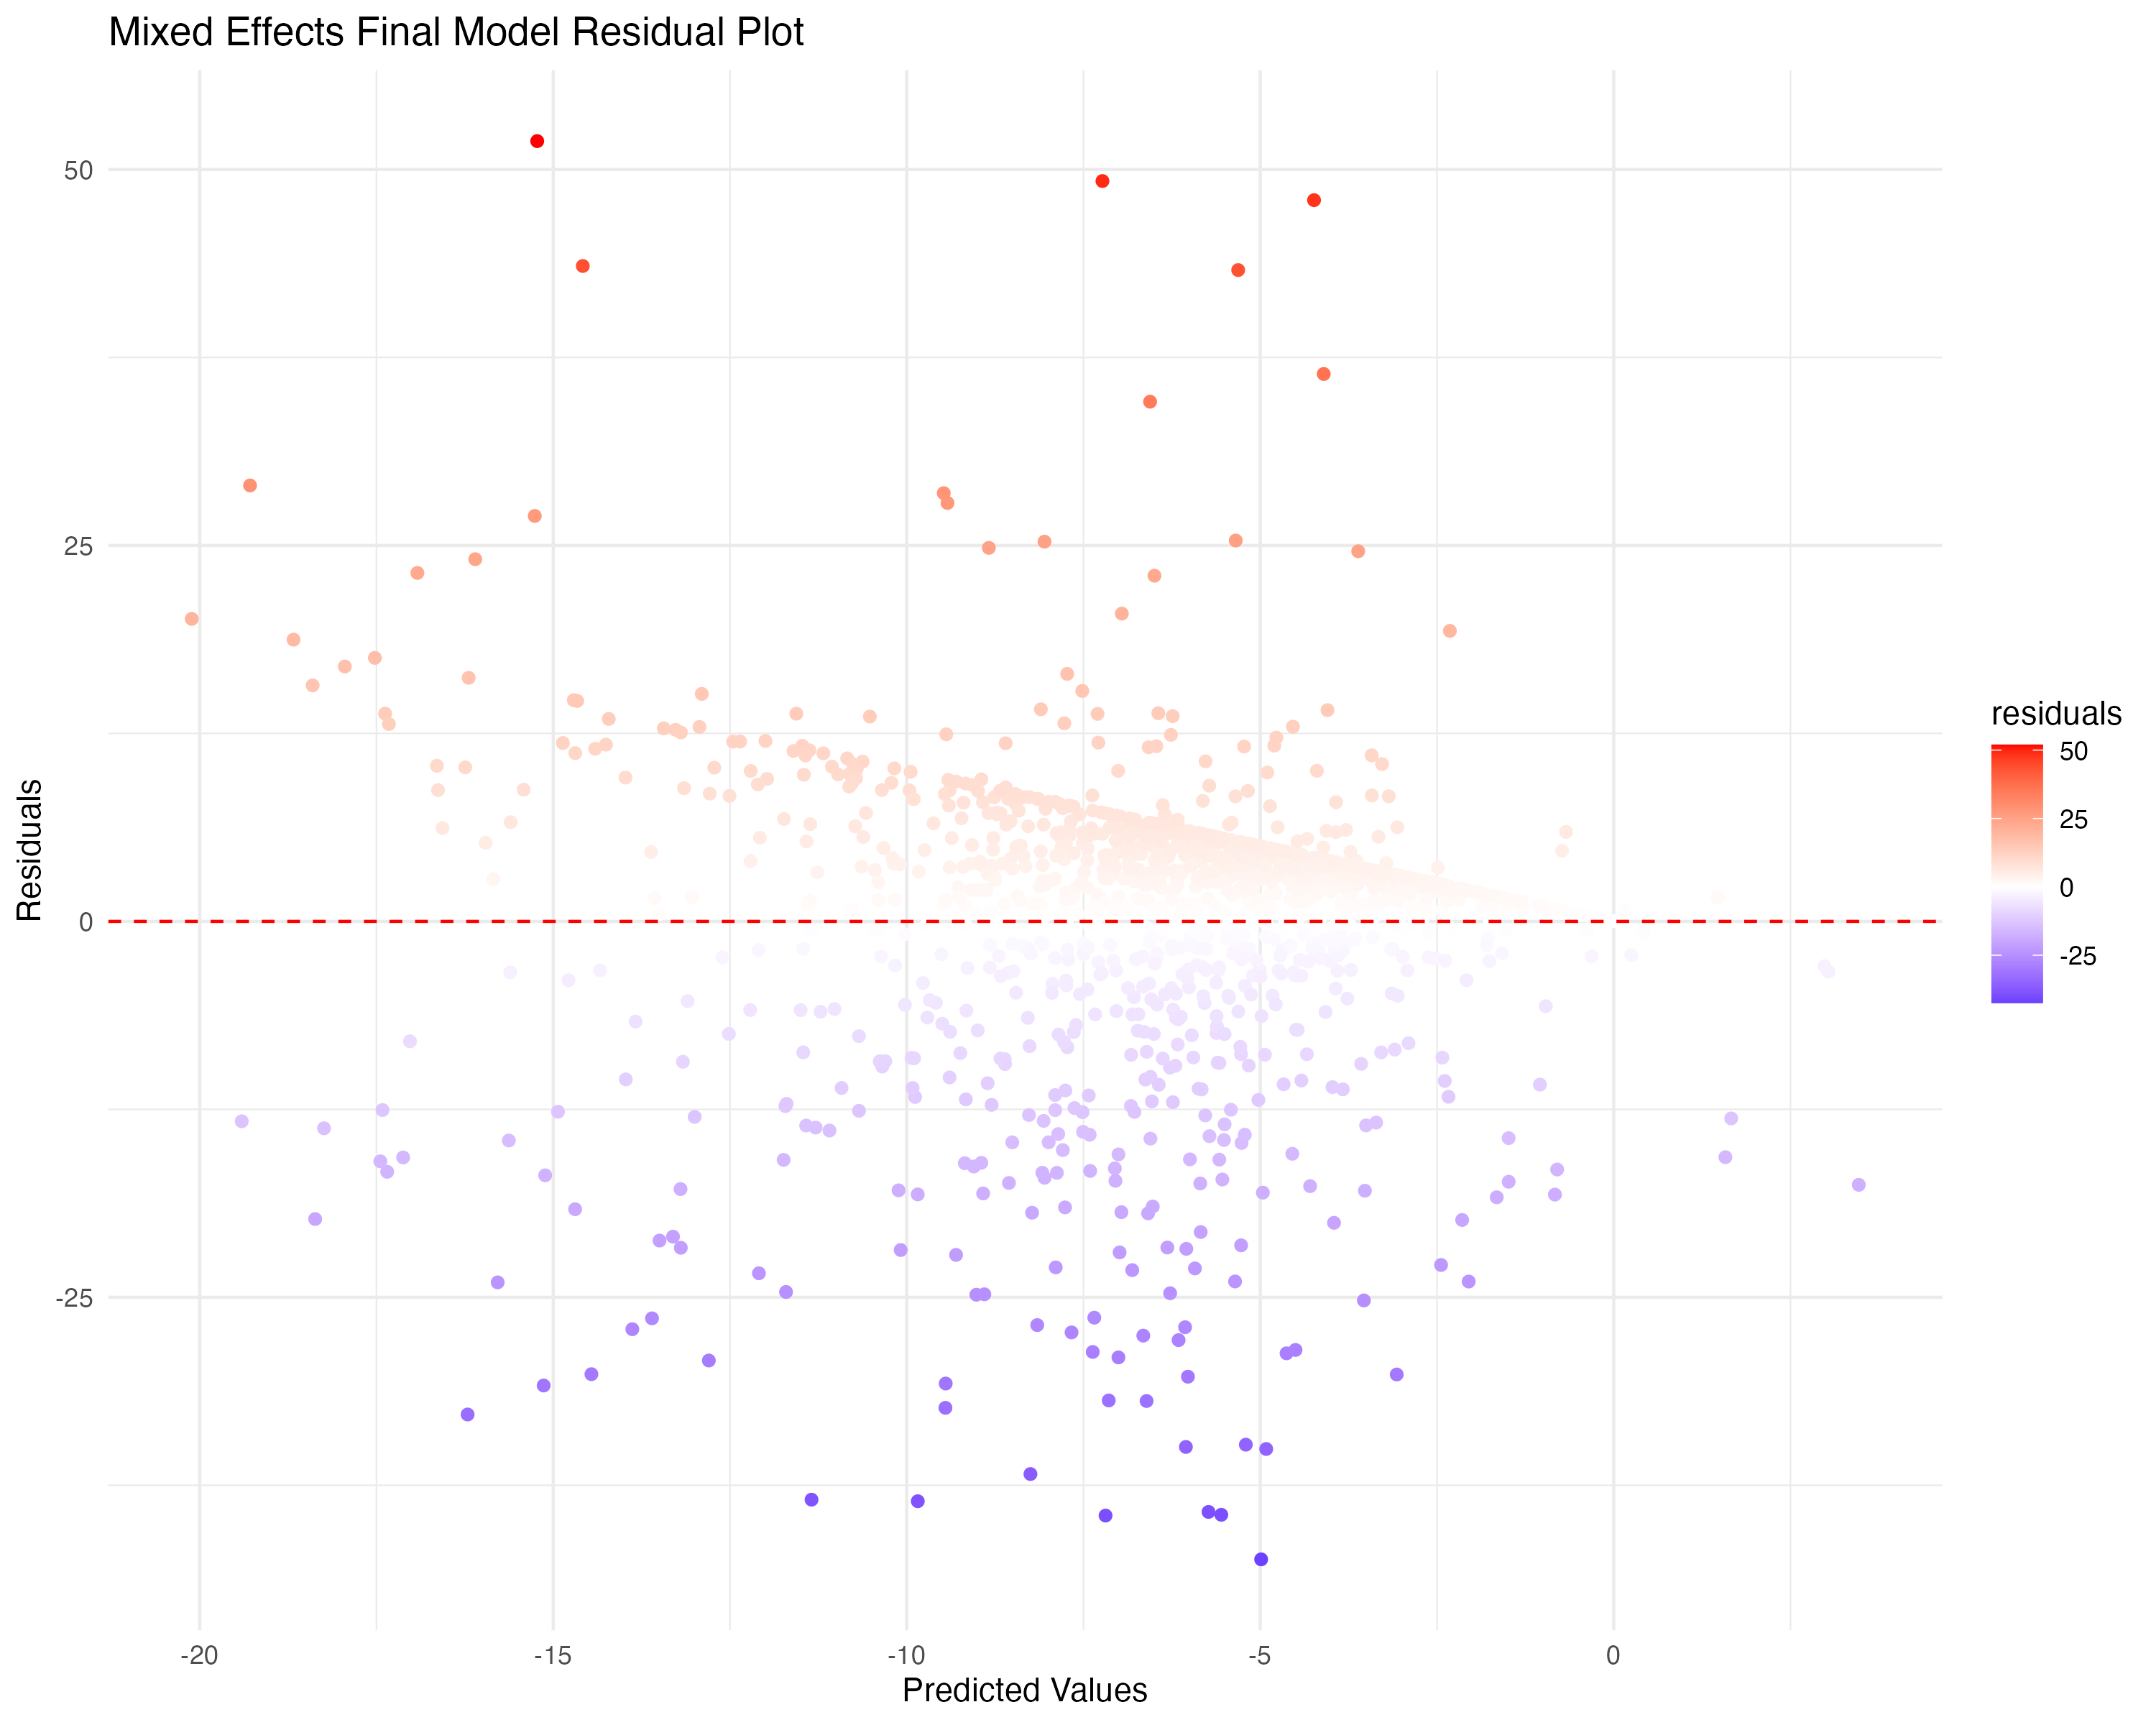
\includegraphics[width=0.8\textwidth]{figures/final_model_residuals.png}
    \caption{Mixed Effects Model Residuals Plot}
    \label{fig:mixed_effects_residuals}
\end{figure}

\section{Finding the best Model}
Using Pycaret, a Machine Learning library, we will be comparing the performance of various models on the dataset. The models will be evaluated based on the RMSE, MAE, and R-squared values. The best model will be selected based on the RMSE value. We used timeseries cross-validation to ensure that the data is split in a time series fashion.The folds are created using the TimeSeriesSplit method from the scikit-learn library. We are not tuning the hyperparameters for the models in this section, as we will be doing that in the next section. This is just to get a sense of how the models perform on the dataset and which models are worth tuning.

% include table
\begin{longtable}{lrrrr}
\caption{Cross Validation Results for All Tested Models}
\label{tab:cross-validated-results}\\
\toprule
                          Model &   MAE &     MSE &  RMSE &     R2 \\
\midrule
\endfirsthead
\caption[]{Cross Validation Results for All Tested Models} \\
\toprule
                          Model &   MAE &     MSE &  RMSE &     R2 \\
\midrule
\endhead
\midrule
\multicolumn{5}{r}{{Continued on next page}} \\
\midrule
\endfoot

\bottomrule
\endlastfoot 
% color 6.91 green
                 Bayesian Ridge &  4.15 &   48.40 &  \textbf{6.91} &   0.09 \\
             CatBoost Regressor &  4.34 &   48.77 &  6.94 &   0.09 \\
               Ridge Regression &  4.22 &   48.74 &  6.94 &   0.08 \\
    Orthogonal Matching Pursuit &  4.29 &   49.09 &  6.96 &   0.08 \\
                    Elastic Net &  4.25 &   49.35 &  6.97 &   0.08 \\
               Lasso Regression &  4.23 &   49.54 &  6.99 &   0.07 \\
   Lasso Least Angle Regression &  4.23 &   49.54 &  6.99 &   0.07 \\
    Gradient Boosting Regressor &  4.34 &   49.57 &  7.00 &   0.07 \\
Light Gradient Boosting Machine &  4.35 &   49.71 &  7.01 &   0.07 \\
        Random Forest Regressor &  4.56 &   50.25 &  7.04 &   0.06 \\
          Extra Trees Regressor &  4.51 &   50.90 &  7.08 &   0.05 \\
                Dummy Regressor &  4.45 &   54.09 &  7.30 &  -0.01 \\
      Extreme Gradient Boosting &  4.85 &   57.20 &  7.51 &  -0.07 \\
          K Neighbors Regressor &  4.80 &   60.37 &  7.71 &  -0.13 \\
                Huber Regressor &  4.38 &   67.05 &  8.13 &  -0.25 \\
        Decision Tree Regressor &  5.89 &   96.97 &  9.80 &  -0.84 \\
             AdaBoost Regressor &  9.13 &  115.14 & 10.60 &  -1.12 \\
   Passive Aggressive Regressor &  6.84 &  187.64 & 12.92 &  -2.66 \\
              Linear Regression & 31.33 & 3024.39 & 35.90 & -42.10 \\
\end{longtable}


\noindent Note how Bayesian Ridge and CatBoost have the lowest RMSE values. We will be exploring these models further in the next section. In general though, no model is significantly better than the others, which suggests that there is significant unexplained variance in the data. This is to be expected, as the CDP survey data is a first step in understanding the decarbonization rate, but there are many other factors that determine the decarbonization rate, especially in the long term. Additionally, there is a lot of noise in the data due to inconsistent reporting, which makes it difficult to predict the decarbonization rate accurately.

\section{Bayesian Ridge Model}

\begin{table}[H]
    \centering
    \caption{Bayesian Ridge Model Performance Metrics for Training and Test Sets}
    \label{tab:bayesian_ridge_performance}
    \begin{tabular}{lcccc}
    \hline
    Set & $R^2$ & RMSE & MSE & MAE \\ 
    \hline
    Training & 0.9 & 6.91 & 48.4 & 4.15 \\
    Test & 0.10 & 9.58 & 91.9 & 6.46 \\
    \hline
    \end{tabular}
\end{table}

% Feature Importance Plot
\begin{figure}[H]
    \centering
    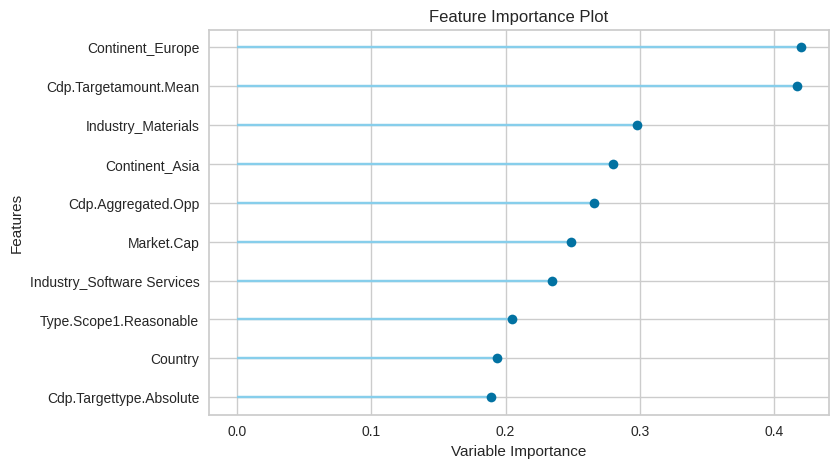
\includegraphics[width=0.8\textwidth]{figures/Bayes_Importance.png}
    \caption{Bayesian Ridge Model Feature Importance Plot}
    \label{fig:bayesian_ridge_feature_importance}
\end{figure}

% Residuals Plot
\begin{figure}[H]
    \centering
    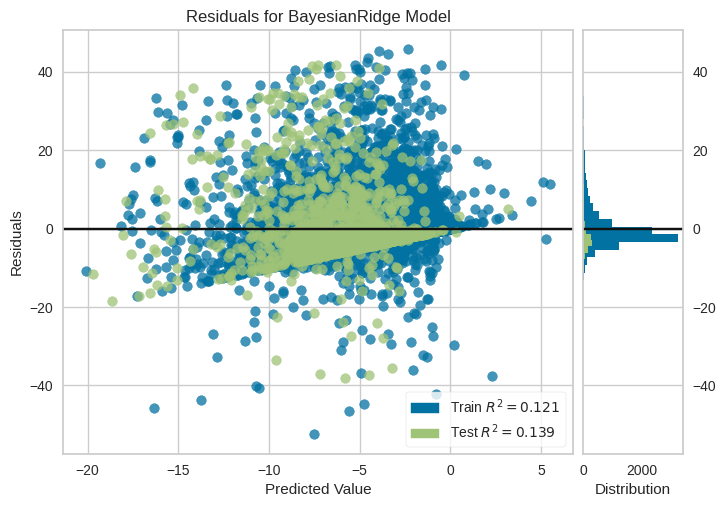
\includegraphics[width=0.8\textwidth]{figures/Bayes_Residuals.png}
    \caption{Bayesian Ridge Model Residuals Plot}
    \label{fig:bayesian_ridge_residuals}
\end{figure}

\section{Catboost Regressor Model}
To tune the Catboost Regressor model, we used grid search and cross-validation to find the best hyperparameters for the model. The hyperparameters that we tuned are the learning rate, the depth of the tree, the number of trees, and the l2 regularization parameter. We used the TimeSeriesSplit method from the scikit-learn library to ensure that the data is split in a time series fashion with number of folds $cv = 3$. The model was evaluated based on the RMSE, MAE, and R-squared values. The best model was selected based on the RMSE value. The hyperparameters that we tuned are as follows:

\subsection*{Hyperparameter Grid}
\begin{table}[h]
\centering
\caption{Grid of Hyperparameters for Catboost Regressor}
\label{tab:hyperparameter_grid}
\begin{tabular}{@{}ll@{}}
\toprule
Parameter       & Values         \\ \midrule
Depth           & 4, 6, 8        \\
Iterations      & 500, 1000      \\
Learning Rate   & 0.01, 0.02, 0.03 \\
L2 Leaf Reg     & 1, 3           \\ \bottomrule
\end{tabular}
\end{table}

\subsection*{Best Hyperparameters}
\begin{table}[h]
\centering
\caption{Best Hyperparameters for Catboost Regressor}
\label{tab:best_hyperparameters}
\begin{tabular}{@{}ll@{}}
\toprule
Parameter       & Value          \\ \midrule
Depth           & 6              \\
Iterations      & 1000           \\
Learning Rate   & 0.02           \\
L2 Leaf Reg     & 1              \\ \bottomrule
\end{tabular}
\end{table}
% make 


\subsection*{Model Performance Metrics}
\begin{table}[H]
    \centering
    \caption{Catboost Regressor Tuned Model Performance Metrics}
    \label{tab:catboost_regressor_performance}
    \begin{tabular}{lcccc}
    \hline
    Set & $R^2$ & RMSE & MSE & MAE \\ 
    \hline
    Training & 0.33 & 5.73 & 35.91 & 3.47 \\
    Test & 0.11 & 9.54 & 91.13 & 6.25 \\
    \hline
    \end{tabular}
\end{table}

\section{Neural Networks}